%     \item conditional independence
%     \item Example for probabilistic state space model: Gaussian random walk
\section{Random variables and expectation}
This chapter collects the probabilistic background used throughout the thesis. The objects of interest are random quantities that take values in $\mathbb{R}^n$, and we describe them through their distributions and through a few numerical summaries. This section reviews random variables, their distributions, and the notions of expectation, variance, and covariance, together with independence and conditioning. These tools are used in every later chapter, and they are also the language in which the Gaussian family of the next section is defined. We assume the reader is familiar with elementary probability and only fix the notation and the facts we need later. The presentation follows \cite[Ch.~2]{murphy:probabilistic_ml_introduction}.

\subsection{Probability spaces and random variables}
The starting point is a probability space, which makes precise the idea of a random experiment and the way probabilities are assigned to its outcomes.

\begin{definition}[Probability space]\label{def:prob_space}
A \emph{probability space} is a triple $(\Omega, \mathcal{F}, \mathbb{P})$, where $\Omega$ is the \emph{sample space} of possible outcomes, $\mathcal{F}$ is a $\sigma$-algebra of subsets of $\Omega$ whose elements are called \emph{events}, and $\mathbb{P}: \mathcal{F} \to [0,1]$ is a \emph{probability measure} with $\mathbb{P}(\Omega) = 1$ that is countably additive, meaning $\mathbb{P}\bigl(\bigcup_i A_i\bigr) = \sum_i \mathbb{P}(A_i)$ for any countable collection of pairwise disjoint events $A_i \in \mathcal{F}$.
\end{definition}

We rarely work with the space $\Omega$ directly. Instead we observe numerical quantities derived from the outcome, which are modeled as random variables.

\begin{definition}[Random variable and random vector]\label{def:random_variable}
A \emph{random vector} is a measurable map $\mathbf{x}: \Omega \to \mathbb{R}^n$. For $n = 1$ it is called a \emph{random variable}. The \emph{distribution} (or law) of $\mathbf{x}$ is the probability measure $P_{\mathbf{x}}$ on $\mathbb{R}^n$ defined by $P_{\mathbf{x}}(B) = \mathbb{P}(\mathbf{x} \in B)$ for measurable sets $B \subseteq \mathbb{R}^n$.
\end{definition}

In all cases relevant to this thesis the distribution admits a \emph{probability density function} $p_{\mathbf{x}}$ with respect to the Lebesgue measure, so that
\begin{equation}\label{eq:density}
    \mathbb{P}(\mathbf{x} \in B) = \int_B p_{\mathbf{x}}(\mathbf{x})\, \mathrm{d}\mathbf{x},
\end{equation}
and we write $\mathbf{x} \sim p_{\mathbf{x}}$, dropping the subscript where the variable is clear from the context. We summarize a distribution through a few key numbers, which we turn to now.

\subsection{Expectation, variance, and covariance}
The expectation is the probability-weighted average value of a random vector and gives the center of its distribution.

\begin{definition}[Expectation]\label{def:expectation}
The \emph{expectation} (or mean) of a random vector $\mathbf{x} \sim p$ is
\begin{equation}\label{eq:expectation}
    \mathbb{E}[\mathbf{x}] = \int_{\mathbb{R}^n} \mathbf{x}\, p(\mathbf{x})\, \mathrm{d}\mathbf{x},
\end{equation}
taken componentwise and defined whenever the integral exists. We write $\boldsymbol{\mu} = \mathbb{E}[\mathbf{x}]$.
\end{definition}

A property we use repeatedly is that expectation is linear. For a deterministic matrix $A \in \mathbb{R}^{m \times n}$, a vector $\mathbf{b} \in \mathbb{R}^m$, and random vectors $\mathbf{x}, \mathbf{y}$ of matching dimension,
\begin{equation}\label{eq:linearity_expectation}
    \mathbb{E}[A\mathbf{x} + \mathbf{b}] = A\,\mathbb{E}[\mathbf{x}] + \mathbf{b}, \qquad
    \mathbb{E}[\mathbf{x} + \mathbf{y}] = \mathbb{E}[\mathbf{x}] + \mathbb{E}[\mathbf{y}].
\end{equation}
The second identity holds whether or not $\mathbf{x}$ and $\mathbf{y}$ are independent.

Linearity also works when the random quantity is a matrix and deterministic matrices multiply it from both sides. For a random matrix $\mathbf{M}$ and deterministic matrices $A$ and $B$ of matching dimensions,
\begin{equation}\label{eq:linearity_matrix}
    \mathbb{E}[A\mathbf{M}B] = A\,\mathbb{E}[\mathbf{M}]\,B.
\end{equation}
The reason is that every entry of $A\mathbf{M}B$ is a fixed linear combination of the entries of $\mathbf{M}$, with coefficients built from $A$ and $B$ alone. Taking the expectation of such a combination gives the same combination of the individual expectations, which is exactly the right hand side. We use this form below whenever a covariance is transformed, since a covariance is the expectation of a matrix rather than of a vector.

While the expectation locates the distribution, the variance and covariance describe how widely it is spread and how its components vary together.

\begin{definition}[Variance and covariance]\label{def:covariance}
The \emph{variance} of a scalar random variable $x$ with mean $\mu$ is $\mathrm{Var}(x) = \mathbb{E}[(x - \mu)^2] \ge 0$, and its square root is the \emph{standard deviation}. For a random vector $\mathbf{x}$ with mean $\boldsymbol{\mu}$, the \emph{covariance matrix} is
\begin{equation}\label{eq:cov_matrix}
    \mathrm{Cov}(\mathbf{x}) = \mathbb{E}\!\left[(\mathbf{x} - \boldsymbol{\mu})(\mathbf{x} - \boldsymbol{\mu})^\top\right] \in \mathbb{R}^{n \times n}.
\end{equation}
\end{definition}

The entry $(i,j)$ of $\mathrm{Cov}(\mathbf{x})$ is the scalar covariance $\mathrm{Cov}(x_i, x_j) = \mathbb{E}[(x_i - \mu_i)(x_j - \mu_j)]$, so the diagonal collects the variances of the components and the off-diagonal entries measure how pairs of components vary together. The covariance matrix is symmetric and positive semidefinite, since for any $\mathbf{a} \in \mathbb{R}^n$ we have $\mathbf{a}^\top \mathrm{Cov}(\mathbf{x})\, \mathbf{a} = \mathrm{Var}(\mathbf{a}^\top \mathbf{x}) \ge 0$. Throughout the thesis we denote the covariance matrix by $\mathbf{P}$.

Expectation and covariance transform in a simple way under affine maps, a fact that underlies the prediction step of the Kalman filter and several of the Gaussian proofs below.

\begin{proposition}[Affine transformation of mean and covariance]\label{prop:affine_moments}
Let $\mathbf{x}$ be a random vector with mean $\boldsymbol{\mu}$ and covariance $\mathbf{P}$, let $A \in \mathbb{R}^{m \times n}$, and let $\mathbf{b} \in \mathbb{R}^m$. Then $\mathbf{y} = A\mathbf{x} + \mathbf{b}$ has
\begin{equation}\label{eq:affine_moments}
    \mathbb{E}[\mathbf{y}] = A\boldsymbol{\mu} + \mathbf{b}, \qquad
    \mathrm{Cov}(\mathbf{y}) = A\,\mathbf{P}\,A^\top.
\end{equation}
\end{proposition}

\begin{proof}
The mean follows from linearity \eqref{eq:linearity_expectation}. For the covariance, $\mathbf{y} - \mathbb{E}[\mathbf{y}] = A(\mathbf{x} - \boldsymbol{\mu})$, so
\[
    \mathrm{Cov}(\mathbf{y}) = \mathbb{E}\!\left[A(\mathbf{x} - \boldsymbol{\mu})(\mathbf{x} - \boldsymbol{\mu})^\top A^\top\right]
    = A\,\mathbb{E}\!\left[(\mathbf{x} - \boldsymbol{\mu})(\mathbf{x} - \boldsymbol{\mu})^\top\right] A^\top
    = A\,\mathbf{P}\,A^\top,
\]
where $A$ and $A^\top$ are pulled out of the expectation by the matrix form of linearity \eqref{eq:linearity_matrix}.
\end{proof}

\subsection{Independence and conditioning}
Two random vectors are \emph{independent} if their joint density factorizes into the product of the marginals,
\begin{equation}\label{eq:independence}
    p(\mathbf{x}, \mathbf{y}) = p(\mathbf{x})\, p(\mathbf{y}).
\end{equation}
Independence implies that the components are uncorrelated, that is $\mathrm{Cov}(\mathbf{x}, \mathbf{y}) = \mathbb{E}[(\mathbf{x} - \boldsymbol{\mu}_x)(\mathbf{y} - \boldsymbol{\mu}_y)^\top] = \mathbf{0}$. As a consequence, the covariance of a sum of independent random vectors is the sum of the covariances,
\begin{equation}\label{eq:cov_sum}
    \mathrm{Cov}(\mathbf{x} + \mathbf{y}) = \mathrm{Cov}(\mathbf{x}) + \mathrm{Cov}(\mathbf{y}),
\end{equation}
a property we rely on when independent noise is added to a state in the models of the following chapters. The converse does not hold in general. Uncorrelated random vectors need not be independent, although for jointly Gaussian vectors the two notions are equivalent. 

When two quantities are dependent, observing one changes our knowledge of the other. This is captured by the conditional distribution. For $p(\mathbf{y}) > 0$ the \emph{conditional density} of $\mathbf{x}$ given $\mathbf{y}$ is
\begin{equation}\label{eq:conditional_density}
    p(\mathbf{x} \mid \mathbf{y}) = \frac{p(\mathbf{x}, \mathbf{y})}{p(\mathbf{y})},
\end{equation}
and the corresponding \emph{conditional expectation} is $\mathbb{E}\left[\mathbf{x}\mid \mathbf{y}\right] = \int_{\mathbb{R}^n} \mathbf{x}\, p\left(\mathbf{x} \mid \mathbf{y}\right)\, \mathrm{d}\mathbf{x}$. The marginal density is recovered by integrating out the other variable, $p(\mathbf{x}) = \int p(\mathbf{x}, \mathbf{y})\, \mathrm{d}\mathbf{y}$. Conditioning on observed quantities is the key operation in Bayesian inference, which we review in Section~\ref{sec: bayesian inference} and apply recursively from Chapter~\ref{chap:bayesian} onward. For jointly Gaussian vectors the conditional distribution is again Gaussian and available in closed form, as shown in Proposition~\ref{prop:conditional}, which is what makes the filters of this thesis tractable.

With these tools in place, we turn to the Gaussian family, on which the rest of the chapter and the filtering algorithms of the later chapters rely.

\section{Gaussian distributions}
The Gaussian (or normal) distribution is central to the filtering methods of this thesis. A Gaussian distribution is fully described by two parameters. The mean determines the center of the distribution, and the variance describes the spread around that center. This two parameter form makes it possible to track a Gaussian belief by propagating only its mean and covariance which is exactly what the recursive filters of the later chapters do. 

Another important property of Gaussian distributions is that they are easy to work with mathematically. The Gaussian family is closed under several operations. The marginal and conditional distributions of a multivariate Gaussian are themselves Gaussian. Moreover, linear transformations and sums of Gaussian variables also produce Gaussian distributions. These properties are especially useful in probabilistic modeling because they allow many inference problems to be solved analytically. 

It is especially useful in state space models and Bayesian filtering, where a Gaussian prior, a Gaussian likelihood, and linear dynamics yield a posterior that remains Gaussian and can be computed in closed form. This is the key reason why algorithms such as the Kalman filter admit efficient recursive solutions~\cite[Ch.~3]{murphy:probabilistic_ml_introduction}.

The Gaussian distribution also has a strong theoretical justification. According to the central limit theorem, the sum of many independent random variables tends to follow a Gaussian distribution, even when the individual variables are not Gaussian. Because many real-world sources of noise arise from the combination of many small independent effects, Gaussian models are often a natural choice when modeling measurement noise or residual errors~\cite[Ch.~2]{murphy:probabilistic_ml_introduction}.

In the following sections we review the main properties of Gaussian distributions. We begin with the one-dimensional Gaussian and then introduce the multivariate case. We also discuss marginal and conditional distributions, sums of Gaussian variables, and affine transformations, all of which are used in the Bayesian filtering methods of the later chapters.

\subsection{The one-dimensional Gaussian}
We begin with the one-dimensional Gaussian distribution. A random variable $x$ follows a Gaussian (or normal) distribution with parameters $\mu$ and $\sigma^2$, written $x \sim \mathcal{N}(\mu, \sigma^2)$ if its probability density function (PDF) is given by:
%
\begin{equation}\label{eq: gaussian pdf 1d}
    p(x) = \frac{1}{\sqrt{2\pi\sigma^2}} \exp\left( -\frac{(x - \mu)^2}{2\sigma^2} \right).
\end{equation}
%
The distribution is fully characterized by the two parameters $\mu$ and $\sigma^2$. These parameters are exactly the mean $\mathbb{E}[x] = \mu$ and variance $\text{Var}(x) = \sigma^2$ of the distribution. The mean determines the location of the distribution, while the variance measures how widely the values of $x$ are spread around the mean~\cite[Ch.~2]{murphy:probabilistic_ml_introduction}.

Figure \ref{fig:1d-gaussian} shows the density \eqref{eq: gaussian pdf 1d} for several values of the standard deviation $\sigma = \sqrt{\sigma^2}$, all centered at the same mean. Each curve is a probability density, so the area under each curve equals one. The Gaussian has a characteristic bell-shaped curve and is symmetric around the mean $\mu$. Values close to the mean occur with higher probability, while values farther away become increasingly unlikely. The standard deviation controls the width of the bell. Around 95\% of the probability mass falls within two standard deviations of the mean~\cite[Ch.~2]{murphy:probabilistic_ml_introduction}.

\begin{figure} 
    \centering
    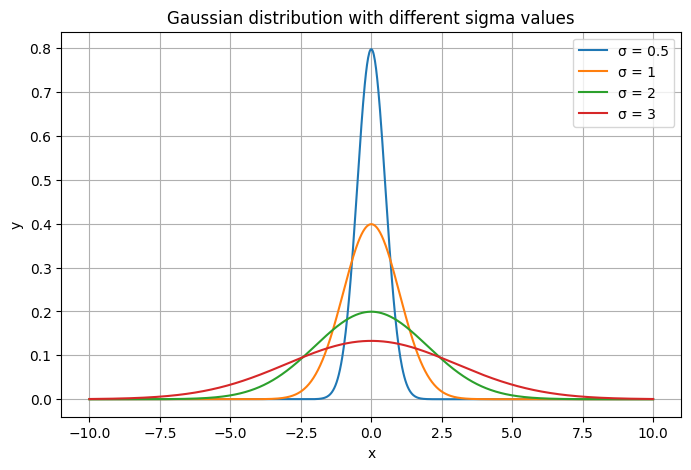
\includegraphics[width=0.5\linewidth]{Figures/Gaussian distributions with different sigma values.png}
    \caption{1D Gaussian distributions with different standard deviations}
    \label{fig:1d-gaussian}
\end{figure}

\subsection{The multivariate Gaussian and joint distribution}
In many practical problems we are interested in several related variables rather than a single scalar quantity. In such cases it is convenient to represent the variables as a random vector. The multivariate Gaussian distribution generalizes the one-dimensional Gaussian to vector-valued random variables. 

Its building block is the standard Gaussian vector. A random vector $\mathbf{Z} \in \mathbb{R}^k$ is called \emph{standard Gaussian}, written $\mathbf{Z} \sim \mathcal{N}(\mathbf{0}, I_k)$, if its $k$ components are independent and each of them follows the one-dimensional Gaussian $\mathcal{N}(0,1)$ of the previous section. Its mean is $\mathbf{0}$ and its covariance matrix is the identity $I_k$, so every component has variance one and different components are uncorrelated. The definition below builds a general Gaussian vector from such a $\mathbf{Z}$ by a linear map and a shift.

\begin{definition}[Gaussian random vector] \label{def:gaussian_vector} 
A random vector $\mathbf{x} \in \mathbb{R}^n$ is called a Gaussian random vector if there exist a matrix $A \in \mathbb{R}^{n \times k}$ and a vector $\boldsymbol{\mu} \in \mathbb{R}^n$ such that 
\[
\mathbf{x} = A\mathbf{Z} + \boldsymbol{\mu},
\]
where $\mathbf{Z} \sim \mathcal{N}(\mathbf{0}, I_k)$ is a standard Gaussian random vector. We write $\mathbf{x} \sim \mathcal{N}(\boldsymbol{\mu},\mathbf{P}),$ where $\mathbf{P} = AA^\top \in \mathbb{R}^{n \times n}$ is the covariance matrix. 
\end{definition} 
% \begin{remark} 
% If the covariance matrix $\mathbf{P}$ is positive definite, then the distribution admits the probability density function 
% \begin{equation} \label{eq:mvn_density}
%     p(\mathbf{x}) = \frac{1}{\sqrt{(2\pi)^n |\mathbf{P}|}} \exp\!\left( -\frac{1}{2} (\mathbf{x}-\boldsymbol{\mu})^\top \mathbf{P}^{-1} (\mathbf{x}-\boldsymbol{\mu}) \right).  
% \end{equation}
When P is singular, the distribution is supported on a lower-dimensional affine subspace and no density with respect to the Lebesgue measure on $\mathbb{R}^n$ exists. Definition~\ref{def:gaussian_vector} covers both cases. 
% \end{remark} 

\begin{remark}\label{rem:mean_cov}
The mean and covariance follow directly from the definition. For $\mathbf{x} = A\mathbf{Z} + \boldsymbol{\mu}$ with $\mathbf{Z} \sim \mathcal{N}(\mathbf{0}, I)$, the mean and covariance follow directly from linearity of expectation:
\[
  \mathbb{E}[\mathbf{x}] = \boldsymbol{\mu}, \qquad
  \mathrm{Cov}(\mathbf{x})
  = \mathbb{E}\!\left[A\mathbf{Z}\mathbf{Z}^\top A^\top\right]
  = A\,\underbrace{\mathbb{E}[\mathbf{Z}\mathbf{Z}^\top]}_{=\,I}\,A^\top
  = AA^\top = \mathbf{P}.
\]
\end{remark}

The covariance matrix $\mathbf{P}$ describes both how much uncertainty there is in each variable and how the variables change together. The diagonal entries of $\mathbf{P}$ represent the marginal variances of each component, while the off-diagonal entries represent the correlations between components. When the off-diagonal terms are zero, the components are independent, and the uncertainty forms an axis-aligned ``cloud'' around the mean. When the off-diagonal terms are nonzero, this cloud becomes tilted, showing that knowing one variable gives us information about the other~\cite[Ch.~3]{murphy:probabilistic_ml_introduction}. This behavior is illustrated in Figure \ref{fig:2d-gaussian}.

\begin{figure} \label{fig:2d-gaussian}
    \centering
    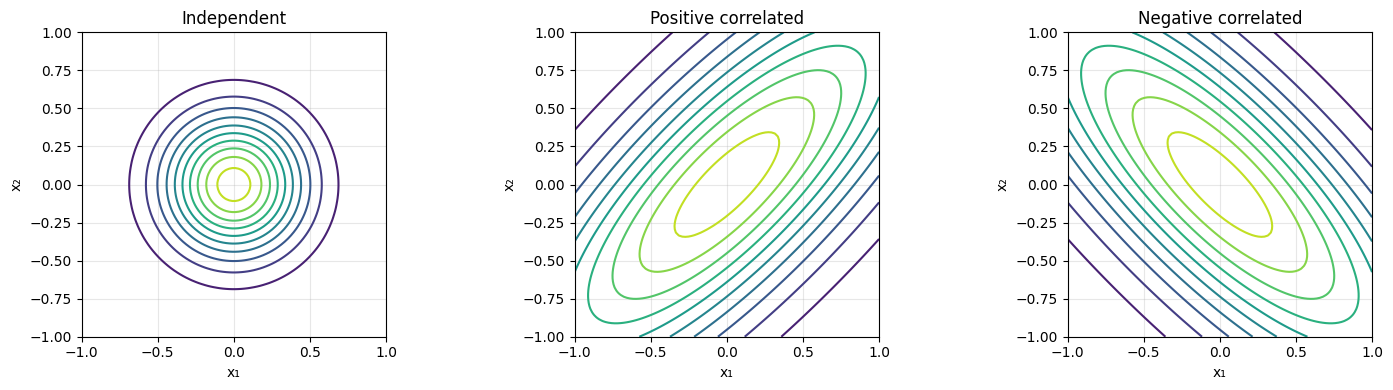
\includegraphics[width=1.0\linewidth]{Figures/Bivariate Gaussian distribution with different covariances.png}
    \caption{Contour plots of bivariate Gaussian distributions with different covariances. From left to right: independent variables, positive correlation and negative correlation.}
\end{figure}


% We will denote multivariate Gaussians as
% \[
% \mathbf{x} \sim \mathcal{N}(\boldsymbol{\mu}, \mathbf{P}),
% \]
% where $\boldsymbol{\mu}$ is the mean vector and $\mathbf{P}$ the covariance matrix. The probability density function (PDF) of the multivariate Gaussian is given by
% \begin{equation}
%     p(\mathbf{x}) =
%     \frac{1}{\sqrt{(2\pi)^n |\mathbf{P}|}}
%     \exp\left(
%     -\frac{1}{2}
%     (\mathbf{x}-\boldsymbol{\mu})^\top
%     \mathbf{P}^{-1}
%     (\mathbf{x}-\boldsymbol{\mu})
%     \right).\label{eq: gaussian pdf nd}
% \end{equation}

% \subsubsection{Marginal and conditional distributions}
In many applications, we are interested only in a subset of the variables, or we want to update our knowledge about one variable after observing another. Gaussian distributions are particularly useful because they allow us to compute marginal and conditional distributions in closed form. We now derive the analytical expressions for these operations.

Consider a jointly Gaussian random vector partitioned into two components
\[
\mathbf{z} :=
\begin{pmatrix}
\mathbf{x} \\
\mathbf{y}
\end{pmatrix}
\:\sim\:
\mathcal{N}
\left(
\begin{pmatrix}
\boldsymbol{\mu}_x \\
\boldsymbol{\mu}_y
\end{pmatrix},
\begin{pmatrix}
\mathbf{P}_{xx} & \mathbf{P}_{xy} \\
\mathbf{P}_{yx} & \mathbf{P}_{yy}
\end{pmatrix}
\right),
\]
where $\boldsymbol{\mu}_x$ and $\boldsymbol{\mu}_y$ are the mean vectors of the two components. The diagonal blocks $\mathbf{P}_{xx} = \mathrm{Cov}(\mathbf{x})$ and $\mathbf{P}_{yy} = \mathrm{Cov}(\mathbf{y})$ are the covariance matrices of $\mathbf{x}$ and $\mathbf{y}$ on their own, and the off-diagonal block $\mathbf{P}_{xy} = \mathrm{Cov}(\mathbf{x}, \mathbf{y}) = \mathbf{P}_{yx}^\top$ records how the two components vary together.

\begin{proposition}[Marginal distribution]\label{prop:marginal}
% The marginal distribution of $\mathbf{x}$ is obtained by selecting the corresponding components of the mean and covariance matrix. In other words,
% \[
% \mathbf{x} \sim
% \mathcal{N}(\mathbf{m}_x, \mathbf{P}_{xx}).
% \]
% Similarly, the marginal distribution of $\mathbf{y}$ is
% \[
% \mathbf{y} \sim
% \mathcal{N}(\mathbf{m}_y, \mathbf{P}_{yy}).
% \]
The marginal distributions of\, $\mathbf{x}$ and\, $\mathbf{y}$ are
\[
\mathbf{x}
\:\sim\:
\mathcal{N}(\boldsymbol{\mu}_x,\mathbf{P}_{xx}),\qquad
\mathbf{y}
\:\sim\:
\mathcal{N}(\boldsymbol{\mu}_y,\mathbf{P}_{yy}).
\]
\end{proposition}
This means that if we are only interested in a subset of the variables, we can ignore the rest without losing the Gaussian form. We just pick the relevant entries of the mean vector and covariance matrix. 
\begin{proof}
Since $\mathbf{z} = (\mathbf{x}, \mathbf{y})^\top$
is Gaussian, by Definition~\ref{def:gaussian_vector} there exist a matrix $A$, a vector $\boldsymbol{\mu}$, and a standard Gaussian vector $\mathbf{Z} \sim \mathcal{N}(\mathbf{0}, I)$ such that $\mathbf{z} = A\mathbf{Z} + \boldsymbol{\mu}$.
Let $B := \begin{bmatrix}I & 0\end{bmatrix}$. Then
\[
\mathbf{x} = B\mathbf{z} 
= B(A\mathbf{Z}+\boldsymbol{\mu})
= BA\mathbf{Z}+B\boldsymbol{\mu}.
\]

By Definition~\ref{def:gaussian_vector}, $\mathbf{x}$ is Gaussian with
\[
  \mathbb{E}[\mathbf{x}] = B\boldsymbol{\mu} = \boldsymbol{\mu}_x, \qquad
  \mathrm{Cov}(\mathbf{x}) = (BA)(BA)^\top = BAA^\top B^\top = B\mathbf{P}B^\top = \mathbf{P}_{xx}.
\]
The result for $\mathbf{y}$ follows analogously with $B = \begin{bmatrix}0 & I\end{bmatrix}$.
\end{proof}


% If the value of $\mathbf{y}$ is observed, we can compute 
The conditional distribution of $\mathbf{x}$ given $\mathbf{y}$ is also Gaussian. 
\begin{proposition}[Conditional distribution, {\cite[Lemma~A.2]{sarkka:bayesian_filtering}}]\label{prop:conditional}
The conditional distribution of\, $\mathbf{x}$ given $\mathbf{y}$ is
\[
  \mathbf{x} \mid \mathbf{y} 
  \;\sim\;
  \mathcal{N}\!\left(\boldsymbol{\mu}_{x|y},\, \mathbf{P}_{x|y}\right),
\]
where
\begin{align}
  \boldsymbol{\mu}_{x|y} &= \boldsymbol{\mu}_x + \mathbf{P}_{xy}\mathbf{P}_{yy}^{-1}(\mathbf{y} - \boldsymbol{\mu}_y),\label{eq:cond_mean}\\
  \mathbf{P}_{x|y} &= \mathbf{P}_{xx} - \mathbf{P}_{xy}\mathbf{P}_{yy}^{-1}\mathbf{P}_{yx}.\label{eq:cond_cov}
\end{align}
\end{proposition}

These expressions show how observing $\mathbf{y}$ updates the estimate of $\mathbf{x}$. The mean shifts according to the difference between the observation and its expected value $\mathbf{y} - \boldsymbol{\mu}_y$, while the covariance decreases, reflecting the reduction in uncertainty after incorporating the new information. As we will see in Chapter~\ref{chap:kalman}, equations \eqref{eq:cond_mean}--\eqref{eq:cond_cov} are precisely the update equations of the Kalman filter.
% \[
% \mathbf{x} \mid \mathbf{y}
% \sim
% \mathcal{N}(\mathbf{m}_{x|y}, \mathbf{P}_{x|y}),
% \]
% where the conditional mean and covariance are
% \[
% \mathbf{m}_{x|y}
% =
% \mathbf{m}_x
% +
% \mathbf{P}_{xy}
% \mathbf{P}_{yy}^{-1}
% (\mathbf{y} - \mathbf{m}_y),
% \]

% \[
% \mathbf{P}_{x|y}
% =
% \mathbf{P}_{xx}
% -
% \mathbf{P}_{xy}
% \mathbf{P}_{yy}^{-1}
% \mathbf{P}_{yx}.
% \]
% These expressions show how the observation $\mathbf{y}$ updates our estimate of $\mathbf{x}$. The mean shifts according to the difference between the observation and its expected value, while the covariance decreases, reflecting the reduction in uncertainty after incorporating the new information~\cite[Ch.~3.2.3]{murphy:probabilistic_ml_introduction}.
% This shows how our uncertainty about $\mathbf{x}_x$ changes once we observe $\mathbf{x}_y$. 

% In the next sections we will see that these Gaussian conditioning formulas form the basis of recursive Bayesian estimation. In particular, they lead directly to the update equations used in the Kalman filter.

% Finally, you can obtain the marginal distribution back from the conditional by integrating out the conditioning variable: 
% \[
% p(\mathbf{x}_x) = \int p(\mathbf{x}_x \mid \mathbf{x}_y) p(\mathbf{x}_y) d\mathbf{x}_y.
% \]
% For Gaussians, this integration results in another Gaussian with mean $\boldsymbol{\mu}_x$ and covariance $\mathbf{P}_{xx}$, consistent with the marginal above.

% \subsubsection{Sum of independent Gaussians} 

\begin{proposition}[Sum of independent Gaussians] \label{prop:sum}
Let $\mathbf{x} \sim \mathcal{N}(\boldsymbol{\mu}_x, \mathbf{P}_x)$ and $\mathbf{y} \sim \mathcal{N}(\boldsymbol{\mu}_y, \mathbf{P}_y)$ be independent.
Then
\[
  \mathbf{x} + \mathbf{y} \; \sim \; \mathcal{N}(\boldsymbol{\mu}_x + \boldsymbol{\mu}_y,\; \mathbf{P}_x + \mathbf{P}_y).
\]
\end{proposition}

\begin{proof}
By Definition~\ref{def:gaussian_vector} write $\mathbf{x} = A_x\mathbf{Z}_x + \boldsymbol{\mu}_x$ and $\mathbf{y} = A_y\mathbf{Z}_y + \boldsymbol{\mu}_y$, where $A_xA_x^\top = \mathbf{P}_x$, $A_yA_y^\top = \mathbf{P}_y$, and $\mathbf{Z}_x \sim \mathcal{N}(\mathbf{0}, I_{l_x})$, $\mathbf{Z}_y \sim \mathcal{N}(\mathbf{0}, I_{l_y})$ are independent standard Gaussian vectors.
Define
\[
  \mathbf{Z}' := \begin{pmatrix}\mathbf{Z}_x\\\mathbf{Z}_y\end{pmatrix}\in \mathbb{R}^{l_x+l_y}.
\]
Since $\mathbf{Z}_x$ and $\mathbf{Z}_y$ are independent standard normals, $\mathbf{Z}' \sim \mathcal{N}(\mathbf{0}, I_{l_x+l_y})$ is also standard normal. Then
\[
  \mathbf{x} + \mathbf{y}
  = \underbrace{\begin{bmatrix}A_x & A_y\end{bmatrix}}_{=:\,A'} \mathbf{Z}' + (\boldsymbol{\mu}_x + \boldsymbol{\mu}_y).
\]
Therefore $\mathbf{x}+\mathbf{y}$ is Gaussian with covariance matrix 
\[
A'(A')^\top = A_xA_x^\top + A_yA_y^\top = \mathbf{P}_x + \mathbf{P}_y.
\]
\end{proof}


% The sum of independent Gaussian random variables is also Gaussian. This allows uncertainty from different sources to be combined while remaining within the Gaussian family.

% Let $\mathbf{x} \in \mathbb{R}^n$ and $\mathbf{y} \in \mathbb{R}^n$ be two independent Gaussian random vectors
% \[
% \mathbf{x} \sim \mathcal{N}(\mathbf{m}_x,\mathbf{P}_x), 
% % \qquad\qquad
% \mathbf{y} \sim \mathcal{N}(\mathbf{m}_y,\mathbf{P}_y),
% \]
% and consider their sum $\mathbf{z} = \mathbf{x} + \mathbf{y}.$
% The mean of $\mathbf{z}$ follows from the linearity of expectation:
% \begin{align*}
% \mathbb{E}[\mathbf{z}]
% &= \mathbb{E}[\mathbf{x} + \mathbf{y}] \\
% &= \mathbb{E}[\mathbf{x}] + \mathbb{E}[\mathbf{y}] \\
% &= \mathbf{m}_x + \mathbf{m}_y.
% \end{align*}
% %
% Moreover, since $\mathbf{x}$ and $\mathbf{y}$ are independent, their covariance matrices add:
% \begin{align*}    
% \mathrm{Cov}(\mathbf{z})
% &= \mathrm{Cov}(\mathbf{x} + \mathbf{y}) \\
% &= \mathrm{Cov}(\mathbf{x}) + \mathrm{Cov}(\mathbf{y}) \\
% &= \mathbf{P}_x + \mathbf{P}_y.
% \end{align*}
% %
% Therefore the sum $\mathbf{z}$ is also Gaussian:
% \begin{equation} \label{sum of gaussians}
% \mathbf{z} \sim 
% \mathcal{N}(\mathbf{m}_x + \mathbf{m}_y,\; \mathbf{P}_x + \mathbf{P}_y).
% \end{equation}



%This result is widely used in dynamical systems where uncertainty from different sources is combined. For example, in state space models the system dynamics often include additive Gaussian process noise. Because Gaussian distributions are closed under addition, the resulting state distribution remains Gaussian, which is a key property exploited by the Kalman filter. \cite[Ch.~3.3]{murphy:probabilistic_ml_introduction}

% \subsection{Affine transformations}
A further useful property of Gaussian distributions is that they are preserved under affine transformations. This will later be used in the prediction step of the Kalman filter.

\begin{proposition}[Affine transformation]\label{prop:affine}
Let $\mathbf{x} \sim \mathcal{N}(\boldsymbol{\mu}, \mathbf{P})$, $C \in \mathbb{R}^{m \times n}$, and $\mathbf{b} \in \mathbb{R}^m$. Then
\begin{equation}\label{eq:affine}
  \mathbf{y} := C\mathbf{x} + \mathbf{b} 
  \:\sim\:
  \mathcal{N}(C\boldsymbol{\mu} + \mathbf{b},\; C\mathbf{P}C^\top).
\end{equation}
\end{proposition}

\begin{proof}
Write $\mathbf{x} = A\mathbf{Z} + \boldsymbol{\mu}$ with $AA^\top = \mathbf{P}$ and $\mathbf{Z} \sim \mathcal{N}(\mathbf{0}, I)$. Then
\[
  \mathbf{y} = C(A\mathbf{Z} + \boldsymbol{\mu}) + \mathbf{b} = \underbrace{(CA)}_{=:\,A'}\mathbf{Z} + \underbrace{(C\boldsymbol{\mu}+\mathbf{b})}_{=:\,\boldsymbol{\mu}'}.
\]
By Definition~\ref{def:gaussian_vector}, $\mathbf{y}$ is Gaussian with $\mathbb{E}[\mathbf{y}] = \boldsymbol{\mu}'$ and $\mathrm{Cov}(\mathbf{y}) = A'(A')^\top = C\mathbf{P}C^\top$.
\end{proof}
Note that Proposition~\ref{prop:marginal} is a special case of Proposition~\ref{prop:affine} with $C = B = \begin{bmatrix}I & 0\end{bmatrix}$ and $\mathbf{b} = \mathbf{0}$. The following joint distribution pattern appears repeatedly in Gaussian state space models and is the key piece for the Kalman filter derivation in Chapter~\ref{chap:kalman}.

\begin{proposition}[Joint distribution]\label{prop:joint}
Suppose $\mathbf{x} \sim \mathcal{N}(\boldsymbol{\mu}, \mathbf{P})$ and
\begin{equation}\label{eq:linear_obs}
  \mathbf{y} := \mathbf{H}\mathbf{x} + \mathbf{u} + \mathbf{r},
  \qquad \mathbf{r} \sim \mathcal{N}(\mathbf{0}, \mathbf{R}),
\end{equation}
with $\mathbf{H} \in \mathbb{R}^{m \times n}$, $\mathbf{u} \in \mathbb{R}^m$, $\mathbf{R} \in \mathbb{R}^{m \times m}$, and $\mathbf{r}$ independent of $\mathbf{x}$. Then

\begin{equation}\label{eq:joint_linear}
  \begin{pmatrix}
  \mathbf{x}\\
  \mathbf{y}
  \end{pmatrix}
  \sim \mathcal{N}\left(
    \begin{pmatrix}
    \boldsymbol{\mu}\\
    \mathbf{H}\boldsymbol{\mu}+\mathbf{u}
    \end{pmatrix},
    \begin{pmatrix}
      \mathbf{P} & \mathbf{P}\mathbf{H}^\top\\
      \mathbf{H}\mathbf{P} & \mathbf{H}\mathbf{P}\mathbf{H}^\top + \mathbf{R}
    \end{pmatrix}
  \right).
\end{equation}
\end{proposition}


\begin{proof}
By Proposition~\ref{prop:affine}, $\mathbf{H}\mathbf{x} + \mathbf{u}$ is Gaussian. By Proposition~\ref{prop:sum}, adding the independent noise $\mathbf{r}$ gives $\mathbf{y} \sim \mathcal{N}(\mathbf{H}\boldsymbol{\mu}+\mathbf{u},\, \mathbf{H}\mathbf{P}\mathbf{H}^\top + \mathbf{R})$.
The cross-covariances follow from $\mathrm{Cov}(\mathbf{x}, \mathbf{y}) = \mathrm{Cov}(\mathbf{x}, \mathbf{H}\mathbf{x}) = \mathbf{P}\mathbf{H}^\top$ and $\mathrm{Cov}(\mathbf{y},\mathbf{x})=\mathbf{H}\mathbf{P}$, using the independence of $\mathbf{x}$ and $\mathbf{r}$. Combining the means, variance, and cross-variances yields the stated joint Gaussian distribution. 
\end{proof}

%This block covariance structure appears frequently in probabilistic state space models and plays an important role in the derivation of Bayesian filtering algorithms such as the Kalman filter~\cite[Ch.~3.3]{murphy:probabilistic_ml_introduction}.

We now show how these patterns work together in a simple tracking problem, a single time step of the kind of model we formalize in the next section.

\begin{example}[One step in a linear Gaussian tracking problem]\label{ex:tracking_1d} % One step Kalman filter
Imagine we are tracking the position and velocity of an object moving along a straight line. The state vector at time $t$ is
\[
\mathbf{x}_t =
    \begin{bmatrix}
    p_t \\
    v_t
    \end{bmatrix}
\in \mathbb{R}^2,
\]
where $p_t$ denotes position and $v_t$ denotes velocity.
Suppose that at time $t$ our current belief about the state is Gaussian
\[
\mathbf{x}_t \sim \mathcal{N}(\mathbf{x}_{t|t},\mathbf{P}_t),
\]
with mean $\mathbf{x}_{t|t} \in \mathbb{R}^2$ and covariance matrix $\mathbf{P}_t \in \mathbb{R}^{2\times2}$. The double index is the notation we keep for the rest of the thesis. A single index means the state itself, so $\mathbf{x}_t$ is the true state, which we do not observe. A double index means an estimate of it, $\mathbf{x}_{t|s} = \mathbb{E}[\mathbf{x}_t \mid \mathbf{y}_{1:s}]$, with the same indices on its covariance $\mathbf{P}_{t|s}$. A colon denotes a block of consecutive times, so $\mathbf{y}_{1:s} = (\mathbf{y}_1,\ldots,\mathbf{y}_s)$ and likewise $\mathbf{x}_{1:t-1}$. Thus $\mathbf{x}_{t|t}$ is the estimate after the measurement at time $t$, and $\mathbf{x}_{t+1|t}$ the estimate of the next state before its measurement arrives.

\textbf{Prediction step:} We now want to predict the state at the next time step $t+1$. Assume the object moves with approximately constant velocity and that the time step between measurements is $\Delta t$. The model can then be written as
\[
\mathbf{x}_{t+1}
=\mathbf{A}\mathbf{x}_t + \mathbf{q}_t,
\qquad
\mathbf{A} :=
    \begin{bmatrix}
    1 & \Delta t \\
    0 & 1
    \end{bmatrix}
\in \mathbb{R}^{2\times2},
\qquad
\mathbf{q}_t \sim \mathcal{N}(\mathbf{0},\mathbf{Q}),
\]
where $\mathbf{q}_t \in \mathbb{R}^2$ represents Gaussian process noise with covariance matrix $\mathbf{Q} \in \mathbb{R}^{2\times2}$.

Using the properties of affine transformations (Proposition~\ref{prop:affine}) and sums of independent Gaussian variables (Proposition~\ref{prop:sum}), the predicted state is again Gaussian:
\[
\mathbf{x}_{t+1} \sim \mathcal{N}(\mathbf{x}_{t+1|t},\mathbf{P}_{t+1|t}),
\]
where

\[
\mathbf{x}_{t+1|t} = \mathbf{A}\mathbf{x}_{t|t},
\]
and
\[
\mathbf{P}_{t+1|t}
=\mathbf{A}\mathbf{P}_t\mathbf{A}^\top + \mathbf{Q}.
\]

\textbf{Update step:} Suppose we receive a noisy measurement of the position at time $t+1$:
\[
\mathbf{y}_{t+1}
=\mathbf{H}\mathbf{x}_{t+1} + \mathbf{r}_{t+1},
\qquad
\mathbf{H} =
    \begin{bmatrix}
    1 & 0
    \end{bmatrix}
\in \mathbb{R}^{1\times2},
\qquad
\mathbf{r}_{t+1} \sim \mathcal{N}(\mathbf{0},\mathbf{R}),
\]
where $\mathbf{r}_{t+1}$ represents measurement noise with covariance $\mathbf{R} \in \mathbb{R}^{1\times1}$.

Since the state and measurement are jointly Gaussian (Proposition~\ref{prop:joint}), the conditional distribution of the state given the measurement is also Gaussian:
\[
\mathbf{x}_{t+1} \mid \mathbf{y}_{t+1} \sim \mathcal{N}(\mathbf{x}_{t+1|t+1},\mathbf{P}_{t+1}),
\]
where
\begin{align*}
    \mathbf{x}_{t+1|t+1} &=\mathbf{x}_{t+1|t}+\mathbf{P}_{t+1|t}\mathbf{H}^\top(\mathbf{H}\mathbf{P}_{t+1|t}\mathbf{H}^\top + \mathbf{R})^{-1}(\mathbf{y}_{t+1} - \mathbf{H}\mathbf{x}_{t+1|t}),\\
    \mathbf{P}_{t+1} &= \mathbf{P}_{t+1|t}-\mathbf{P}_{t+1|t}\mathbf{H}^\top(\mathbf{H}\mathbf{P}_{t+1|t}\mathbf{H}^\top + \mathbf{R})^{-1}\mathbf{H}\mathbf{P}_{t+1|t}.
\end{align*}

This simple example already contains the main ingredients of the Kalman filter, a prediction step based on a linear Gaussian transition model followed by an update step obtained from Gaussian conditioning.
Intuitively, we first predict the next state using the model. Then we correct that prediction using the new measurement. Both steps remain in the Gaussian family and so can be fully described by the way they transform the mean and covariance.
\end{example}


\section{Probabilistic state space models}\label{sec: state space model}
% Definition is from the book Bayesian filtering and smoothing` by Simo Särkkä page 51.
The tracking example of the previous section covered a single time-step. We began with a Gaussian belief about the state, predicted the state at the next time, and corrected the prediction with one measurement. However, most estimation problems extend over many time steps. The state keeps evolving and new measurements keep arriving. To describe such a problem we need a model that fixes, for every time step, both how the state changes and how a measurement depends on the state. This is the probabilistic state space model. Every filter developed in the following chapters is defined on a model of this form. We follow the presentation in Chapter~4 of \cite{sarkka:bayesian_filtering}.

\begin{definition}[Probabilistic state space models]\label{def:ssm}
A probabilistic state space model or non-linear filtering model consists of a sequence of conditional probability distributions: 
\begin{align}
    &\mathbf{x}_t \sim p(\mathbf{x}_t \mid \mathbf{x}_{t-1}), \nonumber \\
    &\mathbf{y}_t \sim p(\mathbf{y}_t \mid \mathbf{x}_t),
\end{align}
for $t=1,2, \dots$, where 
\begin{itemize}
    \item[(i)] $\mathbf{x}_t \in \mathbb{R}^n$ is the \textit{state} of the system at time step $t$.
    \item[(ii)] $\mathbf{y}_t \in \mathbb{R}^m$ is the \textit{measurement} (observation) at time step $t$. 
    \item[(iii)] $p(\mathbf{x}_t\mid \mathbf{x}_{t-1})$ is the \textit{transition model} (dynamic model) which describes the stochastic dynamics of the system. The transition model can be a probability density, a counting measure or a combination of them depending on whether the state $\mathbf{x}_t$ is continuous, discrete, or hybrid. 
    \item[(iv)] $p(\mathbf{y}_t\mid \mathbf{x}_t)$ is the \textit{measurement model}, which is the distribution of measurements given the state. 
\end{itemize}
%
The state space model is assumed to be \textit{Markovian}, which means that the evolution of the system depends only on the current state and not on the full history of the process.
\end{definition}

% Property is from the book Bayesian filtering and smoothing` by Simo Särkkä page 52.
\begin{property}[Markov property of states]
The states $\{\mathbf{x}_t\}_{t\geq0}$ form a Markov sequence (or Markov chain if the state is discrete). This means that given $\mathbf{x}_{t-1}$, the state $\mathbf{x}_t$ is independent of any state or observation that happened earlier: 

\begin{equation}\label{prop: Markov property of states}
   p(\mathbf{x}_t\mid \mathbf{x}_{1:t-1},\mathbf{y}_{1:t-1} )=  p(\mathbf{x}_t\mid \mathbf{x}_{t-1}).
\end{equation}
%
Similarly, the past is conditionally independent of the future given the present state: 

\begin{equation}
   p(\mathbf{x}_{t-1}\mid \mathbf{x}_{t:T},\mathbf{y}_{t:T} )=  p(\mathbf{x}_{t-1}\mid \mathbf{x}_t).
\end{equation}
\end{property}

% Property is from the book Bayesian filtering and smoothing` by Simo Särkkä page 52.
\begin{property}[Conditional independence of measurements]
An analogous property holds for measurements. In particular, the current measurement $\mathbf{y}_t$ is conditionally independent of the measurement and state histories given the current state: 

\begin{equation}\label{prop: Conditional independence of measurements}
p(\mathbf{y}_t \mid \mathbf{x}_{1:t}, \mathbf{y}_{1:t-1}) = p(\mathbf{y}_t \mid \mathbf{x}_t).    
\end{equation}
Hence, once the current state is known, the measurement does not depend on earlier states or measurements.
\end{property}

Properties~\eqref{prop: Markov property of states} and \eqref{prop: Conditional independence of measurements} together provide the conditional independence structure that makes the Bayesian filtering recursion of Chapter~\ref{chap:bayesian} valid and tractable. The full measurement history is summarized by the current filtering distribution, so it never needs to be stored explicitly.

\begin{example}[Tracking a drone's position and velocity in 2D]\label{ex:drone}
This example takes the tracking problem of Example~\ref{ex:tracking_1d} from one dimension to two, and follows it over a whole sequence of time steps instead of a single one. Consider a drone flying over an open field. We wish to track its position and velocity in both the horizontal and vertical directions. Since these four quantities describe everything we need to know about the drone's motion, we organize them into a state vector:
\[ 
\mathbf{x}_t = 
\begin{bmatrix}
    p_{x,t} \\ 
    p_{y,t} \\ 
    v_{x,t} \\ 
    v_{y,t} 
\end{bmatrix} \in \R^{4},
\]
where $(p_{x,t}, p_{y,t})$ is the drone's position and $(v_{x,t}, v_{y,t})$ its
velocity at time $t$. 

\textbf{Observation model:} Suppose we have a GPS sensor that provides us with the drone's position at each time step. This means we can measure the position, but not the velocity. In other words, we know where the drone is but not how fast it is moving. The observation model describes how the measurements we receive are connected to the drone's actual position (data we can observe) and velocity (important but hidden variable from direct measurement). 

The observation model is written as: 
\begin{equation}\label{eq: drone observation}
\mathbf{y}_t = \mathbf{H}\mathbf{x}_{t}+\mathbf{r}_{t}, 
\qquad 
\mathbf{r}_t \sim \mathcal{N}(\mathbf{0}, \mathbf{R})
\end{equation}
where $\mathbf{y}_t$ is the measurement at time step $t$, $\mathbf{H}$ is a matrix that shows how the state vector relates to the observed measurements and $\mathbf{r}_t$ represents random measurement noise. In our example, this corresponds to the GPS error. 

The observation matrix in this example is: 
\[
\mathbf{H} = 
\begin{bmatrix}
   1 & 0 & 0 & 0\\
   0 & 1 & 0 & 0\\   
\end{bmatrix}.
\]
The non-zero entries of $\mathbf{H}$ in the first two columns select the position components of the state:
\[
\mathbf{y}_t = 
\begin{bmatrix}
   p_{x,t} \\
   p_{y,t} \\ 
\end{bmatrix} 
+ \mathbf{r}_t.
\]
Therefore, the velocity is a latent (hidden) variable that cannot be observed directly.


\textbf{Transition model:} We assume the drone flies with approximately constant velocity. This means its future position depends only on where it is now and how fast it is going. The position alone would not be enough because the drone might be hovering in place or racing across the field. To account for slight deviations from the ideal model, we add a small amount of Gaussian process noise to the model. In our example, this could represent effects like wind pushing the drone off course. The same type of process noise can also be used to model unknown changes in the drone's velocity.

%This state transition model accounts for small random deviations from constant velocity, with small random deviations. It tells us how the drone's state changes from moment to moment. We include some randomness since movement is not always perfect, e.g.~the wind might push the drone a little off course. 

The transition model can thus be written as: 
\begin{equation}\label{eq: transition model}
    \mathbf{x}_t = \mathbf{A}\mathbf{x}_{t-1}+\mathbf{q}_{t-1}, 
    \qquad 
    \mathbf{q}_{t-1} \sim \mathcal{N}(\mathbf{0}, \mathbf{Q})  
\end{equation}
where $\mathbf{x}_t$ is the state at time step $t$, $\mathbf{A}$ is a matrix that describes how position and velocity are updated and $\mathbf{q}_{t-1}$ represents process noise. 

The transition matrix in this example is
\begin{equation}\label{eq:drone transition}
\mathbf{A}=
\begin{pmatrix}
    1 & 0 & \Delta t & 0 \\
    0 & 1 & 0 & \Delta t \\
    0 & 0 & 1 & 0 \\
    0 & 0 & 0 & 1    
\end{pmatrix},
\end{equation}
where $\Delta t$ is the time step between measurements. In principle, the process noise $\mathbf{q}_{t-1}$ can affect both the position or the velocity. In the following we will consider the special cases where it only affects one or the other.

\begin{itemize}

    \item{\textbf{Position noise only.}}
    Uncertainty arises mainly from small random displacements in the drone's position, while the velocity is assumed to remain constant between time steps. The noise vector takes the form
    \[
    \mathbf{q}_{t-1} = 
    \begin{bmatrix}
        q_{p,x} \\
        q_{p,y} \\
        0 \\
        0
    \end{bmatrix},
    \]
    
    where $q_{p,x},q_{p,y} \sim \mathcal{N}(0,\sigma_{\text{pos}}^2)$ with 
    covariance matrix
    \[
    \mathbf{Q} =
    \begin{bmatrix}
        \sigma_\text{pos}^2 & 0 & 0 & 0 \\
        0 & \sigma_\text{pos}^2 & 0 & 0 \\
        0 & 0 & 0 & 0 \\
        0 & 0 & 0 & 0 
    \end{bmatrix}
    \]
    In this case, the drone moves add a random walk step after moving according to the fixed velocity. This results in a trajectory with sharp edges.  
    
    \item{\textbf{Velocity noise only.}}
    This time we assume the position evolves smoothly but the drone's velocity or direction may change slightly, for example due to a breeze. The noise vector is
    \[
    \mathbf{q}_{t-1}= \begin{bmatrix}
        0 \\
        0 \\
        q_{v,x} \\
        q_{v,y}
    \end{bmatrix}
    \]
     with process noise covariance
    \[
      \mathbf{Q} = \begin{bmatrix}
        0 & 0 & 0 & 0 \\
        0 & 0 & 0 & 0 \\
        0 & 0 & \sigma^{2}_{vel} & 0 \\
        0 & 0 & 0 & \sigma^{2}_{vel}
      \end{bmatrix}.
    \]
    Here the drone follows a smooth trajectory whose direction changes gradually. This model captures more realistic trajectories than the random walk trajectories from above.
\end{itemize}

Before discussing the simulated trajectories, it is important to distinguish between states and observations. In a state space model, the state $\mathbf{x}_t$ is typically not directly observable. Instead, we only observe noisy measurements $\mathbf{y}_t$ generated by the observation model \eqref{eq: drone observation}. For this reason, the state variables are often referred to as \emph{hidden states} or \emph{latent states}. When a state space model is simulated forward in time, we generate a sequence of hidden states by repeatedly applying the transition model \eqref{eq: transition model}. Once the states have been generated, observations can be obtained from the observation model. In the present example, we focus on the hidden state trajectory itself in order to understand how different choices of process noise influence the system dynamics.

To illustrate the effect of the two noise models, we simulate the state space model forward in time. Starting from the initial state
$\mathbf{x}_0 =
\begin{pmatrix}
    0, 0, 1, 0.4
\end{pmatrix}^{\top},$
the hidden states are generated by repeatedly applying the transition model \eqref{eq: transition model} for $T=60$ time steps with $\Delta t = 1$.

Figure~\ref{fig:drone_traj} shows one simulated trajectory for each choice of process noise. In the first case, the noise acts directly on the position while the velocity remains constant between time steps. This produces a jagged trajectory that resembles a random walk. In the second case, the noise acts on the velocity. Since the position is obtained by integrating the velocity over time, small perturbations accumulate gradually and lead to a smooth, curved trajectory.

This example illustrates how different choices of the process noise model can lead to different behaviour, even though the underlying state space model remains the same.

\begin{figure} \label{fig:drone_traj}
    \centering
    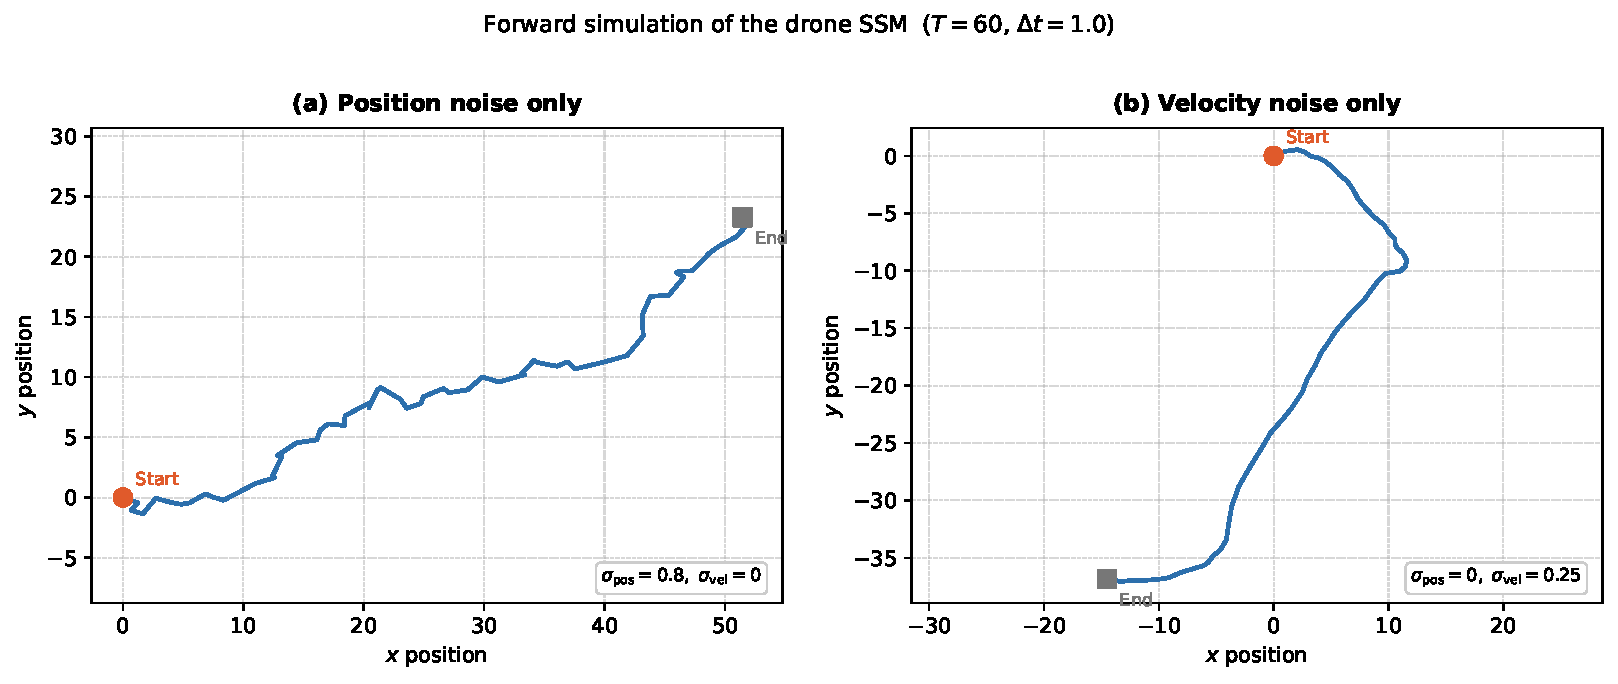
\includegraphics[width=\textwidth]{Figures/Drone trajectories forward simulation.pdf} 
    \caption{Forward simulation of the drone state space model ($T = 60$, $\Delta t = 1$). Left: position noise only ($\sigma_{\mathrm{pos}} = 0.8$), resulting in a jagged, random walk like trajectory. Right: velocity noise only ($\sigma_{\mathrm{vel}} = 0.25$), resulting in a smooth, gradually curving trajectory.}
\end{figure}

% This example illustrates the main components of a probabilistic state space model. The state transition model describes how the hidden state evolves over time, while the observation model connects the hidden state to the measurements. In the following chapters we will develop methods for estimating the hidden state $\mathbf{x}_t$ from the sequence of observations $\mathbf{y}_{1:t}$.
\end{example}

The state space model specifies how states and measurements are generated. Given a state, it tells us the distribution of the next state and of the measurement. In practice we face the reverse problem. We observe the measurements and want to recover the hidden states that produced them. Turning observations into statements about hidden states is the task of Bayesian inference, which we review next in the static setting before applying it recursively over time in Chapter~\ref{chap:bayesian}.


\section{Bayesian inference}\label{sec: bayesian inference}

% Bayesian inference represents beliefs as probability distributions and turns learning into a process of updating probabilities. Every time new data arrive, the prior belief becomes the new posterior, which then serves as the prior for the next update. This recursive idea forms the foundation of Bayesian filtering, where we use new sensor data to continuously improve our estimates of a system’s changing state.
% The idea: Bayesian inference provides a formal framework for updating our beliefs as new evidence becomes available. Answers an intuitive question: ``Given what I already know and what I have just observed, what should I now believe?'' This process is how we naturally learn. 

Bayesian inference provides a systematic way to update our beliefs when new information becomes available. Instead of representing unknown quantities as fixed values, Bayesian methods describe uncertainty using probability distributions. Suppose we want to estimate an unknown quantity $\theta$ using observed data $D$. Before seeing any data, we already have some belief about the possible values of $\theta$, represented by the \emph{prior distribution} $p(\theta)$. Once we observe data, we update this belief using Bayes' theorem. The theorem is not an extra assumption. It follows directly from the definition of a conditional density. Writing the joint density $p(\theta, D)$ in the two ways $p\left(\theta \mid D\right)\, p(D)$ and $p\left(D \mid \theta\right)\, p(\theta)$ and equating them gives the statement below.
\begin{theorem}[Bayes' theorem]\label{thm:bayes}
Let $\theta$ and $D$ be random quantities with joint density $p(\theta, D)$, and assume $p(D) > 0$. Then
    \begin{equation}
      p(\theta \mid D)
      \;=\; \frac{p(D \mid \theta)\, p(\theta)}{p(D)}. \label{eq:bayes}
    \end{equation}
\end{theorem}

Each factor in \eqref{eq:bayes} has a clear interpretation:
\begin{enumerate}
    \item \textbf{Prior distribution} $p(\theta)$: This term represents our belief about $\theta$ before we see the data $D$. If we have little prior information, we can use a vague prior.
    \item \textbf{Likelihood} $p(D \mid \theta)$: The likelihood expresses how probable the observed data $D$ is, assuming a specific value of the parameter $\theta$. The question it answers is ``How likely is it to observe this data if the parameter takes a particular value?''
    \item \textbf{Posterior distribution $p(\theta \mid D)$}: This is the target quantity we want to compute in the Bayesian analysis. It represents our updated belief about the parameter $\theta$ after seeing the data $D$. It answers the question: ``How probable are the values of $\theta$ after seeing the new evidence?''
    \item \textbf{Normalization constant $p(D)$}: This ensures the posterior distribution sums (discrete case) or integrates (continuous case) to 1.  
\end{enumerate}

In many applications the normalization constant is difficult to compute explicitly. For this reason Bayes' theorem is often written in proportional form
\[
\text{Posterior} \propto \text{ Likelihood } \times \text{ Prior},
\]
The symbol $\propto$ means ``is proportional to''. This tells us that our updated belief (the posterior) is a combination of what we thought before (the prior) and what the data is telling us (the likelihood).


\begin{example}
 Let's consider a self-driving car navigating through a city.
\begin{enumerate}
    \item \textbf{Prior belief}: The internal map (prior knowledge) tells the car that the upcoming road is a straight two-lane highway. Based on this belief it should stay in its lane and maintain speed. 
    \item \textbf{New evidence}: Suddenly, the car's sensors, e.g., the cameras, detect a large stationary object in its lane about 100 meters ahead. This is the new data. The likelihood function evaluates this new evidence: ``What is the probability of seeing this sensor reading if the road is clear (very low) and what is the probability if there is a real obstacle (very high)'' 
    \item \textbf{Updated belief}: The car combines its initial map knowledge with the new sensor data. This results in a new updated belief. The prior belief of a clear road is replaced by the posterior belief of an obstructed road, triggering an immediate action. Based on this, the car makes a decision to slow down and safely change lanes. 
\end{enumerate}
\end{example} 
In this example the update happens once. Bayesian filtering, which we develop in the next chapter, applies exactly this update repeatedly over time. At every time step the current belief about the hidden state plays the role of the prior, the new measurement provides the likelihood, and the resulting posterior becomes the prior for the next step.
